\documentclass[10pt,a4paper]{article}
\usepackage{amsmath}
\usepackage[utf8]{vietnam}
\usepackage{amsfonts}
\usepackage{amssymb}
\usepackage{graphicx}
\usepackage{float}
\usepackage{multicol}
\usepackage{tkz-tab}
\usepackage{colortbl}
\usepackage[left=2cm,right=2cm,top=2cm,bottom=2cm]{geometry}
\setlength{\parindent}{0pt}
\begin{document}
\fontsize{18}{30}\selectfont
{\centering TRƯỜNG ĐẠI HỌC CÔNG NGHỆ THÔNG TIN \\
KHOA KHOA HỌC MÁY TÍNH \\
BÀI TẬP MÔN PHÂN TÍCH VÀ THIẾT KẾ THUẬT TOÁN
\par}
\vspace{0.5 cm}
\begin{center}
    \begin{figure}[htp]
     \centering
\includegraphics[scale=.3]{images/logo_uit.jpg} \\
    \end{figure}
    \vspace{1 cm}
    
    \par\noindent\rule{\textwidth}{0.5pt}
    \fontsize{14}{30}\selectfont
    {\centering \textbf{HOMEWORK \#02 \\
    GIẢI PHƯƠNG TRÌNH ĐỆ QUY BẰNG NHIỀU PHƯƠNG PHÁP} \\
    }
    \par\noindent\rule{\textwidth}{0.5pt}
    
    \fontsize{14}{30}\selectfont
    \begin{tabbing}
    \hspace{2 in} \= \hspace{2 in} \= \kill

    Môn: \> Phân tích thiết kế thuật toán \\
    Lớp: \> CS112.N23.KHCL \\
    Giảng viên hướng dẫn: \> Huỳnh Thị Thanh Thương \\
    Nhóm thực hiện: \> Hồ Thị Khánh Hiền(Leader) - 21522057 \\
    \hspace{5.3 cm}Tống Trần Tiến Dũng - 21521983 \\
    \hspace{5.3 cm}Bùi Mạnh Hùng - 21522110 \\
    \end{tabbing}  

    \begin{center}
    \fontsize{14}{30}\selectfont
     TP Hồ Chí Minh,{\today}
    \end{center}
\end{center}
\newpage
\fontsize{13}{15}\selectfont
\tableofcontents
\newpage
%write table of contents without Index
%Ex: 
% Bài 1
\section*{Bài tập 1: Thành lập phương trình đệ quy} 
\addcontentsline{toc}{section}{Bài tập 1: Thành lập phương trình đệ quy}
\subsection*{a)}
\addcontentsline{toc}{subsection}{a)}
\begin{figure}[H]
    \centering
    
\includegraphics[scale=0.6]{images/1a.png}
    % \caption{Caption}
    \label{fig:my_label}
\end{figure}
$
T(n) = 
    \begin{cases}
        C_1, \text{ khi n = 0} \\
        T(n-1) + C_2, \text{ khi n > 0}
    \end{cases}
$
\subsection*{b)}
\addcontentsline{toc}{subsection}{b)}
\begin{figure}[H]
    \centering
    
\includegraphics[scale=0.6]{images/1b.png}
    % \caption{Caption}
    \label{fig:my_label}
\end{figure}
$
T(n) = 
    \begin{cases}
        C_1, \text{ khi n $\leq$ 1} \\
        T(n-1) + T(n-2) + C_2, \text{ khi n > 1}
    \end{cases}
$
\subsection*{c)}
\addcontentsline{toc}{subsection}{c)}
\begin{figure}[H]
    \centering
    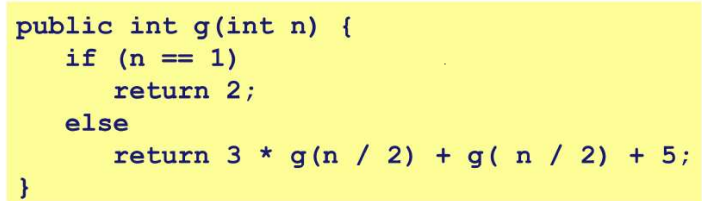
\includegraphics[scale=0.6]{images/1c.png}
    % \caption{Caption}
    \label{fig:my_label}
\end{figure}
$
T(n) = 
    \begin{cases}
        C_1, \text{ khi n $=$ 1} \\
        2T(\frac{n}{2}) + C_2, \text{ khi n > 1}
    \end{cases}
$
\subsection*{d)}
\addcontentsline{toc}{subsection}{d)}
\begin{figure}[H]
    \centering
    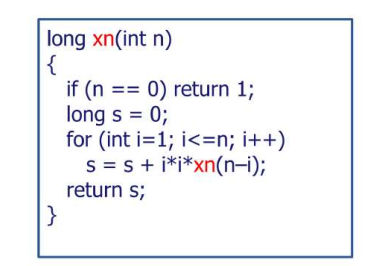
\includegraphics[scale=1]{images/1d.png}
    % \caption{Caption}
    \label{fig:my_label}
\end{figure}
$
T(n) = 
    \begin{cases}
        C_1, \text{ khi n = 0} \\
        \sum_{i=1}^{n}{[T(n-i) + (n-i)C_2]} + C_3, \text{ khi n > 0}
    \end{cases}
$
\subsection*{e)}
\addcontentsline{toc}{subsection}{e)}
\begin{figure}[H]
    \centering
    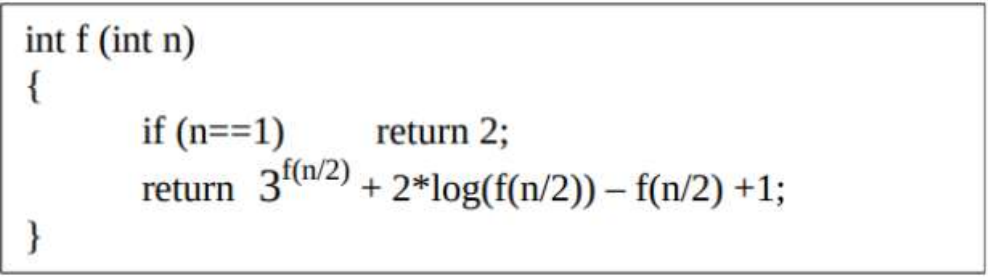
\includegraphics[scale=.6]{images/1e.png}
    % \caption{Caption}
    \label{fig:my_label}
\end{figure}
$
T(n) = 
    \begin{cases}
        C_1, \text{ khi n = 1} \\
        3T(n/2) + C_2, \text{ khi n > 1}
    \end{cases}
$
\subsection*{f)}
\addcontentsline{toc}{subsection}{f)}
\begin{figure}[H]
    \centering
    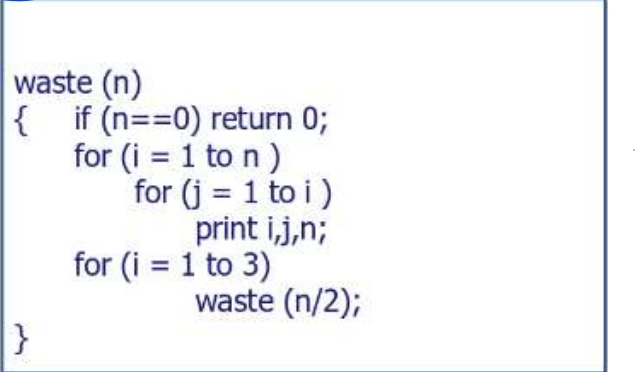
\includegraphics[scale=.7]{images/1f.png}
    % \caption{Caption}
    \label{fig:my_label}
\end{figure}
$
T(n) = 
    \begin{cases}
        C_1, \text{ khi n = 0} \\
        3T(\frac{n}{2}) + \frac{n(n+1)}{2} + C_2, \text{khi $n>0$}
    \end{cases}
$
\subsection*{g)}
\addcontentsline{toc}{subsection}{g)}
\begin{figure}[H]
    \centering
    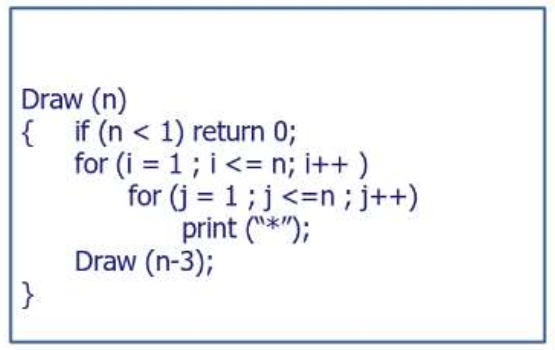
\includegraphics[scale=.7]{images/1g.png}
    % \caption{Caption}
    \label{fig:my_label}
\end{figure}
$
T(n) = 
    \begin{cases}
        C_1, \text{ khi n < 1} \\
        T(n-3) + n^2 + C_2, \text{khi $n\geq1$}
    \end{cases}
$
\subsection*{h)}
\addcontentsline{toc}{subsection}{h)}
\begin{figure}[H]
    \centering
    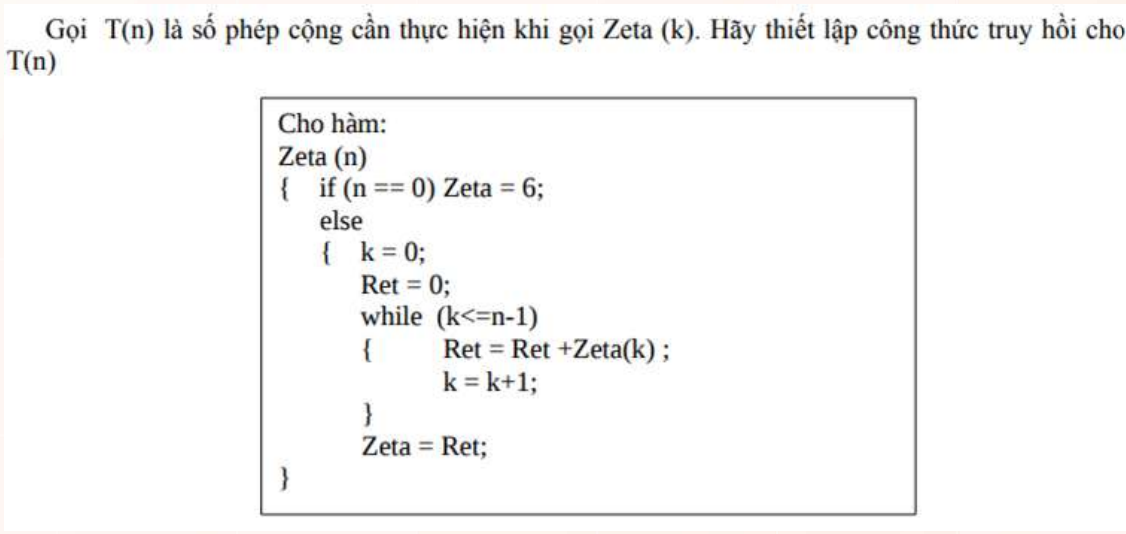
\includegraphics[scale=.7]{images/1h.png}
    % \caption{Caption}
    \label{fig:my_label}
\end{figure}
$
T(n) = 
    \begin{cases}
        0, \text{ khi n = 0} \\
        \sum_{k=0}^{n-1}T(k) + 2n, \text{khi n> 0}
    \end{cases}
$ \\
\textbf{Giải pt đệ quy: } \\
Có: \\
T(0) = 0 \\
T(1) = T(0) + 2.1 = 2 \\
T(2) = $\sum_{k=0}^{1}{T(k)}$ + 2n = T(0) + T(1) + 2.2 = 6 \\
T(3) = T(0) + T(1) + T(2) + 2.3 = 14 \\ ... \\
$\Rightarrow$ T(n) = $\sum_{i=1}^{n}{2^i}$ = $2^{n+1}$ - 2 \\
\textbf{Khi đó: }\\
$
T(n) = 2^{n+1} - 2, \forall n \Rightarrow T(n) = O(2^n)
$ \\
\subsection*{i)}
\addcontentsline{toc}{subsection}{i)}
\begin{figure}[H]
    \centering
    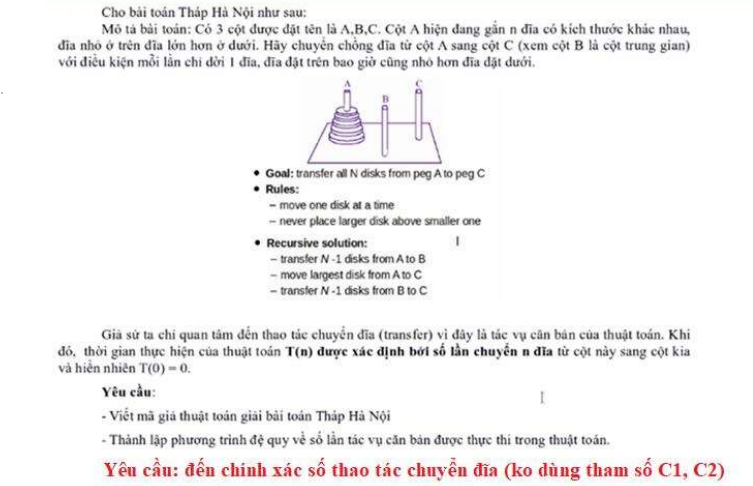
\includegraphics[scale=.7]{images/1i.png}
    % \caption{Caption}
    \label{fig:my_label}
\end{figure}
Bắt đầu giải thuật Tháp Hà nội Hanoi(n, A, C, B)\\
Nếu chỉ có 1 đĩa, di chuyển đĩa từ cột A tới cột C\\
IF n == 1, thì
      di chuyển đĩa từ A tới C  \\   

Nếu có nhiều hơn 1 đĩa:\\

Bước 1: Di chuyển n-1 đĩa từ cột A tới cột B\\
 Hanoi(n - 1, A, B, C)\\
Bước 2: Di chuyển đĩa thứ n từ cột A tới cột C\\

Bước 3: Di chuyển n-1 đĩa từ cột B về cột C\\
Hanoi(n - 1, B, C, A) \\
$
T(n) = 
    \begin{cases}
        1, \text{ khi n = 1} \\
        2T(n-1) + 1, \text{khi $n>1$}
    \end{cases}
$
\subsection*{j)}
\addcontentsline{toc}{subsection}{j)}
\begin{figure}[H]
    \centering
    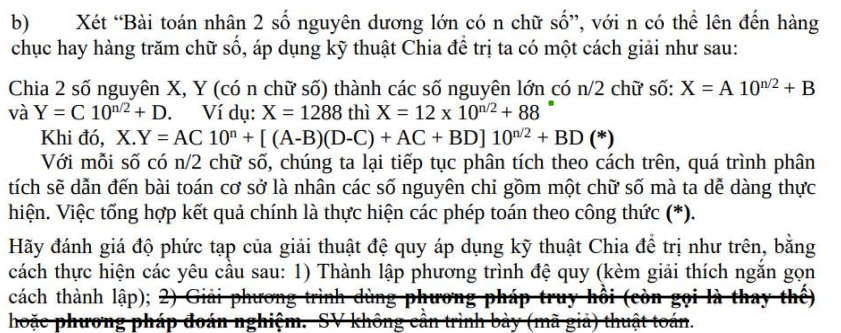
\includegraphics[scale=.7]{images/1j.png}
    % \caption{Caption}
    \label{fig:my_label}
\end{figure}

\text{Từ (*) ta quy ước:}\\
\begin{itemize}
    \item Nếu A,B,C,D là số có $\frac{n}{2}$ chữ số thì (A-B) và (D-C) cũng là số có $\frac{n}{2}$ chữ số \\
    \item AC lặp lại 2 lần trong công thức, ta chỉ gọi đệ quy 1 lần và gán giá trị cho biến x => thế x = AC vào (*) \\
    \item BD lặp lại 2 lần trong công thức, ta chỉ gọi đệ quy 1 lần và gán giá trị cho biến y => thế y = BD vào (*) \\
\end{itemize}
 \\
\text{Khi đó (*) => }
\begin{cases}
    x = AC \\
    y = BD \\
    XY = x.10^n+[(A-B)(D-C)+x+y]10^{\frac{n}{2}}+y \\
\end{cases}
\\
$
T(n) = 
    \begin{cases}
        1, \text{ khi n = 1} \\
        3T(\frac{n}{2}) + C_1, \text{khi $n>1$}
    \end{cases}
$


% Bài 2
\section*{Bài tập 2: Giải các phương trình đệ quy bằng phương pháp truy hồi} 
\addcontentsline{toc}{section}{Bài tập 2: Giải các phương trình đệ quy bằng phương pháp truy hồi}
\subsection*{1)}
\addcontentsline{toc}{subsection}{1)}
\begin{figure}[H]
    \centering
    
\includegraphics[scale=.6]{images/21.png}
    % \caption{Caption}
    \label{fig:my_label}
\end{figure}
T(n) = $T(n-2)+10 = T(n-3) + 15 = T(n-i) + 5i$ \\
Quá trình dừng lại khi đạt tới T(1) $\Rightarrow$ n - i = 1 $\Rightarrow$ i = n -1 \\
\textbf{Khi đó:}
\\
T(n) = T(1) + 5(n-1) = 5n - 5
\subsection*{2)}
\addcontentsline{toc}{subsection}{2)}
\begin{figure}[H]
    \centering
    
\includegraphics[scale=.7]{images/2.2.png}
    % \caption{Caption}
    \label{fig:my_label}
\end{figure}
T(n) = $[T(n-2)+(n-1)]+n = [T(n-3) + (n-2)] +(n-1)+n =T(n-i) + \sum_{k=0}^{i-1}(n-k= T(n-i) + \sum_{k=0}^{i-1}(n)- \sum_{k=0}^{i-1}(k) = T(n-i)+(i-1)n-\frac{(i-1)(i-2)}{2}$\\
......\\
\\
Quá trình kết thúc khi: $n-i = 1 => i = n-1$ \\
\textbf{Khi đó:}
\\
\text{T(n)}
$=T(1) + n(n-2) + \frac{(n-2)(n-3)}{2}\\$
$=1+\frac{(n-2)(n+3)}{2}$\\
$\Rightarrow T(n)=O(n^2)$
\subsection*{3)}
\addcontentsline{toc}{subsection}{3)}
\begin{figure}[H]
    \centering
    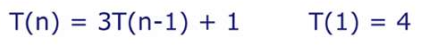
\includegraphics[scale=.7]{images/23.png}
    % \caption{Caption}
    \label{fig:my_label}
\end{figure}
T(n) = $3[3T(n-2)+1]+1 = 9[3T(n-3) + 1] +3+1 = 3^3T(n-3) + 3^2 + 3^1 + 3^0 $\\
......\\
T(n) = $3^iT(n-i)+\sum_{k=0}^{i-1}{3^k}$ \\ \\
$
T(n) = 
    \begin{cases}
        4, \text{ khi n = 1} \\
        3^iT(n-i)+\sum_{k=0}^{i-1}{3^k} , \text{khi $n>1$}
    \end{cases}
$
\\
Quá trình kết thúc khi: $n-i = 1 => i = n-1$ \\
\textbf{Khi đó:}
\\
\text{T(n)}
$=4.3^{n-1} + \sum_{k=0}^{n-2}{3^k}$ 
$=\frac{4}{3}.3^n + 1+ \frac{3^{n-1}-3}{2}$ 
$=\frac{3^{n+1}}{2} - \frac{1}{2}$
\subsection*{4)}
\addcontentsline{toc}{subsection}{4)}
\begin{figure}[H]
    \centering
    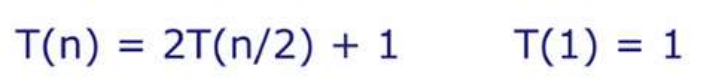
\includegraphics[scale=.6]{images/24.png}
    % \caption{Caption}
    \label{fig:my_label}
\end{figure}
\text{T(n)}
      = 2[2T(n/4)+1] + 1 = 4T(n/4) + 3 = 8T(n/8) + 7 = iT(n/i) + (i-1) \\
Quá trình dừng lại khi đạt tới T(1) $\Rightarrow$ n/i = 1 $\Rightarrow$ i = n \\
\textbf{Khi đó:}
\\
T(n) = nT(1) + n-1 = 2n - 1
\subsection*{5)}
\addcontentsline{toc}{subsection}{5)}
\begin{figure}[H]
    \centering
    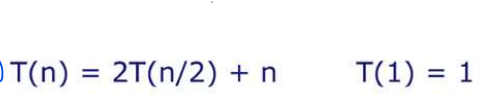
\includegraphics[scale=.7]{images/2.5.png}
    % \caption{Caption}
    \label{fig:my_label}
\end{figure}
T(n) 
$=2[2T(\frac{n}{4}) + (\frac{n}{2})] + n$ 
$=4[2T(\frac{n}{8}) + (\frac{n}{4})] + 2n$ 
$=8T(\frac{n}{8}) + 3n$ 
$= 2^3.T(\frac{n}{2^3}) + 3n$\\
......\\
T(n) = $2^iT(\frac{n}{2^i})+\sum_{k=0}^{i}{n}$ \\ 
= $2^iT(\frac{n}{2^i})+in$\\
\\
Quá trình kết thúc khi: $\frac{n}{2^i} = 1 => i = \log_{2}n$ \\
\textbf{Khi đó:}
\\
\text{T(n)}
$=2^{\log_{2}n} + n\log_{2}n$ 
$=n + n\log_{2}n$ = O(n\log_2(n))$
\subsection*{6)}
\addcontentsline{toc}{subsection}{6)}
\begin{figure}[H]
    \centering
    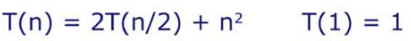
\includegraphics[scale=.7]{images/26.png}
    % \caption{Caption}
    \label{fig:my_label}
\end{figure}
T(n) 
$=2[2T(\frac{n}{4}) + (\frac{n}{2})^2] + n^2$ $=4[2T(\frac{n}{8}) + (\frac{n}{4})^2] + \frac{n^2}{2} + n^2$ $= 2^3.T(\frac{n}{2^3}) + \frac{n^2}{2^2} + \frac{n^2}{2^1} + \frac{n^2}{2^0}$\\
......\\
T(n) = $2^iT(\frac{n}{2^i})+\sum_{k=0}^{i-1}{\frac{n^2}{2^k}}$ \\ \\
$
T(n) = 
    \begin{cases}
        1, \text{ khi n = 1} \\
        2^iT(\frac{n}{2^i})+\sum_{k=0}^{i-1}{\frac{n^2}{2^k}} , \text{khi $n>1$}
    \end{cases}
$
\\
Quá trình kết thúc khi: $\frac{n}{2^i} = 1 => i = \log_{2}n$ \\
\textbf{Khi đó:}
\\
\text{T(n)}
$=2^{\log_{2}n} + n^2.\sum_{k=0}^{\log_{2}n-1}{(\frac{1}{2})^k}$ 
$=n + n^2.2[1-(\frac{1}{2})^{\log_{2}n}]$ 
$=n + 2n^2(1-\frac{1}{n})$
$=2n^2-n$
\subsection*{7)}
\addcontentsline{toc}{subsection}{7)}
\begin{figure}[H]
    \centering
    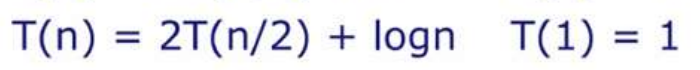
\includegraphics[scale=.7]{images/27.png}
    % \caption{Caption}
    \label{fig:my_label}
\end{figure}
\begin{align*}
    \text{T(n)}
    & = 2[2T(\frac{n}{4})+log(\frac{n}{2})] + logn = 4T(\frac{n}{4}) + 2log(\frac{n}{2}) + logn \\
    & = 4[2T(\frac{n}{8})+log(\frac{n}{4})] + 2log(\frac{n}{2}) + logn \\ 
    & = 8T(\frac{n}{8}) + 4log(\frac{n}{4})+ 2log(\frac{n}{2}) + logn \\
    & = 2^iT(\frac{n}{2^i})+ \sum_{k=0}^{i-1}{2^klog\frac{n}{2^k}}
\end{align*}
\text{Quá trình dừng lại khi đạt tới T(1)}$\Rightarrow n/2^i = 1 \Rightarrow i = log_2{n} = logn$ (\text{$log = log_2$})\\
\begin{align*}
    \text{T(n)} 
    & = n + \sum_{k=0}^{logn-1}{2^klog\frac{n}{2^k}} = n+ logn.\sum_{k=0}^{logn-1}{2^k} - \sum_{k=0}^{logn-1}{2^klog2^k} \\
    & = n + (n-1)logn -log2\sum_{k=0}^{logn-1}{k2^k}  = n + (n-1)logn - log2\big((logn-2)n + 2\big) \\
    & = n + (n-1)logn - nlogn + 2n - 2 = 3n - 2 -logn 
\end{align*}
% Bài 3
\section*{Bài tập 3: Giải các phương trình đệ quy bằng PP truy hồi với T(1) = 1} 
\addcontentsline{toc}{section}{Bài tập 3: Giải các phương trình đệ quy bằng PP truy hồi với T(1) = 1}
\subsection*{1)}
\addcontentsline{toc}{subsection}{1)}
\begin{figure}[H]
    \centering
    
\includegraphics[scale=.7]{images/3,1.png}
    % \caption{Caption}
    \label{fig:my_label}
\end{figure}
T(n) 
$=3[3T(\frac{n}{4}) + (\frac{n}{2})^2] + n^2$ $=3^2[3T(\frac{n}{8}) + (\frac{n}{4})^2] + 3\big(\frac{n}{2}\big)^2+n^2$ 
$= 3^3.T(\frac{n}{2^3}) +3^2\big(\frac{n}{4}\big)^2+3\big(\frac{n}{2}\big)^2+n^2\\$
......\\
$T(n) = 3^i.T(\frac{n}{2^i})+n^2\sum_{k=0}^{i-1}(3^k\frac{1}{2^{2k}})$  \\
$ = 3^i.T(\frac{n}{2^i})+n^2\sum_{k=0}^{i-1}(\frac{3}{4})k$  \\
$ = 3^i.T(\frac{n}{2^i})+n^2\frac{(3/4)^i-1}{(3/4)-1}$  \\

Quá trình kết thúc khi: $\frac{n}{2^i} = 1 => i = \log_{2}n$ \\
\textbf{Khi đó:}
\\
\text{T(n)}
$= 3^{\log_{2}n}+n^2\frac{(3/4)^{\log_{2}n} -1}{(3/4)-1}$ 
$= O(n^2)$ 
\subsection*{2)}
\addcontentsline{toc}{subsection}{2)}
\begin{figure}[H]
    \centering
    
\includegraphics[scale=.7]{images/32.png}
    % \caption{Caption}
    \label{fig:my_label}
\end{figure}
T(n) 
$=8[8T(\frac{n}{4}) + (\frac{n}{2})^3] + n^3$ $=8^2[8T(\frac{n}{8}) + (\frac{n}{4})^3] + 2n^3$ $= 8^3.T(\frac{n}{2^3}) + 3.n^3\\
......\\
$T(n) = $8^i.T(\frac{n}{2^i})+i.n^3$ \\ \\
$
T(n) = 
    \begin{cases}
        1, \text{ khi n = 1} \\
        8^i.T(\frac{n}{2^i})+i.n^3 , \text{khi $n>1$}
    \end{cases}
$
\\
Quá trình kết thúc khi: $\frac{n}{2^i} = 1 => i = \log_{2}n$ \\
\textbf{Khi đó:}
\\
\text{T(n)}
$= 8^{\log_{2}n}+{\log_{2}n}.n^3$ 
$= n^3 + n^3.{\log_{2}n}$ 
\subsection*{3)}
\addcontentsline{toc}{subsection}{3)}
\begin{figure}[H]
    \centering
    
\includegraphics[scale=.6]{images/33.png}
    % \caption{Caption}
    \label{fig:my_label}
\end{figure}
$
\text{T(n)} = 4[4T(\frac{n}{9})+\frac{n}{3}] + n = 16T(\frac{n}{9}) + \frac{7n}{3} \\
= 16[4T(\frac{n}{27})+\frac{n}{9}] + \frac{7n}{3} = 64T(\frac{n}{27}) + \frac{37n}{9} \\ 
= 64[4T(\frac{n}{81})+\frac{n}{27}] + \frac{37n}{9} = 256T(\frac{n}{81}) + \frac{175n}{27} \\
= 4^iT(\frac{n}{3^i}) + \sum_{k=0}^{i-1}{\big(\frac{4}{3}\big)^k}$ \\
Quá trình dừng lại khi đạt tới T(1) $\Rightarrow \frac{n}{3^i} = 1 \Rightarrow i = log_3{n}$ \\
\textbf{Khi đó: }\\
T(n) = $4^{log_3{n}} + \sum_{k=0}^{log_3{n}-1}{\big(\frac{4}{3}\big)^k} = 4^{log_3{n}} + 3\big(\frac{4^{log_3{n}}}{n}-1\big)$
\subsection*{4)}
\addcontentsline{toc}{subsection}{4)}
\begin{figure}[H]
    \centering
    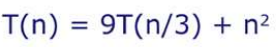
\includegraphics[scale=.7]{images/3.4.png}
    % \caption{Caption}
    \label{fig:my_label}
\end{figure}
T(n) 
$=9[9T(\frac{n}{9}) + (\frac{n}{3})^2] + n^2$ $=9^2[9T(\frac{n}{27}) + (\frac{n}{9})^2] + 2n^2$ 
$= 9^3.T(\frac{n}{3^3}) +3n^2\\$
......\\
$T(n) = = 9^i.T(\frac{n}{3^i}) +in^2\\$ \\

Quá trình kết thúc khi: $\frac{n}{3^i} = 1 => i = \log_{3}n$ \\
\textbf{Khi đó:}
\\
\text{T(n)}
$= 9^{\log_{3}n}T(1)+n^2long_{3}$ 
$= 9+n^2long_{3}$ 
$= O(n^2)$ 
\subsection*{5)}
\addcontentsline{toc}{subsection}{5)}
\begin{figure}[H]
    \centering
    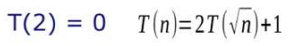
\includegraphics[scale=.7]{images/35.png}
    % \caption{Caption}
    \label{fig:my_label}
\end{figure}
T(n) 
$=2[2T(n^{\frac{1}{4}}) + 1] + 1$ $=2^2[2T(2^{\frac{1}{8}})+1] + 2 + 1$ $= 2^3.T(n^{\frac{1}{2^3}}) + 4 + 2 + 1\\$
......\\
T(n) = $2^i.T(n^{\frac{1}{2^i}}) + \sum_{k=0}^{i-1}2^k$ \\ \\
$
T(n) = 
    \begin{cases}
        0, \text{ khi n = 2} \\
        2^i.T(n^{\frac{1}{2^i}}) + \sum_{k=0}^{i-1}2^k , \text{khi $n>2$}
    \end{cases}
$
\\
Quá trình kết thúc khi: $n^{\frac{1}{2^i}} = 1 => n = 2^{2^i} => i = \log_{2}(\log_{2}n)$ \\
\textbf{Khi đó:}
\\
\text{T(n)}
$= \log_{2}n.0 + 2^i-1 = \log_{2}n -1$ 
% Bai 4
\section*{Bài tập 4: Giải phương trình đệ quy sau dùng phương trình đặc trưng} 
\addcontentsline{toc}{section}{Bài tập 4: Giải phương trình đệ quy sau dùng phương trình đặc trưng}
\subsection*{a)}
\addcontentsline{toc}{subsection}{a)}
\begin{figure}[H]
    \centering
    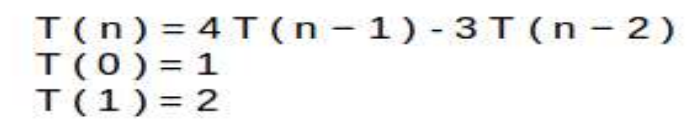
\includegraphics[scale=.9]{images/4a.png}
    % \caption{Caption}
    \label{fig:my_label}
\end{figure}
Xét phương trình T(n) - 4T(n-1) + 3T(n-2) = 0 \\
\text{Đặt} $X^n$ = T(n) \\
\text{Ta có:} $X^n - 4X^{n-1} + 3X^{n-2} = 0 \\
\text{Phương trình đặc trưng: } X^2 - 4X + 3 = 0 \Rightarrow (X-3)(X-1)=0$ \\
Có 2 nghiệm đơn $X_1 = 1$ và $X_2 = 3$ \\
\text{Ta có: T(n) = } $c_1X_1^n + c_2X_2^n$ = $c_1.1 + c_2.3^n$ \\
$\begin{cases}
    T(0) = 1 \\
    T(1) = 2
\end{cases} \Rightarrow
\begin{cases}
    c_1 + c_2 = 1 \\
    c_1 + 3c_2 = 2
\end{cases} \Rightarrow
\begin{cases}
    c_1 = 1/2 \\
    c_2 = 1/2
\end{cases}$\\
Vậy T(n) = $\frac{1}{2} + \frac{3^n}{2}$
\subsection*{b)}
\addcontentsline{toc}{subsection}{b)}
\begin{figure}[H]
    \centering
    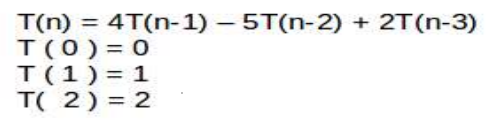
\includegraphics[scale=1]{images/4b.png}
    % \caption{Caption}
    \label{fig:my_label}
\end{figure}
Xét phương trình T(n) - 4T(n-1) + 5T(n-2) + 2T(n-3) = 0 \\
\text{Đặt} $X^n$ = T(n) \\
\text{Ta có:} $X^n - 4X^{n-1} + 5X^{n-2} + 2X^{n-3} = 0 \\
\text{Phương trình đặc trưng: } X^3 - 4X^2 + 5X - 2 =0 \Rightarrow (X-1)^2(X-2) = 0$ \\
Có 1 nghiệm đơn $X_1 = 2$ và nghiệm kép $X_2 = 1$ \\
\text{Ta có: T(n) = } $c_1X_1^n + c_2X_2^n + c_3nX_2^n$= $c_1.2^n + c_2.1^n + c_3n1^n$ \\
$\begin{cases}
    T(0) = 0 \\
    T(1) = 1\\
    T(2) = 2
\end{cases} \Rightarrow
\begin{cases}
    c_1 + c_2 = 0 \\
    2c_1 + c_2 + c_3 = 1\\
    4c_1 + c_2 + 2c_3 = 2
\end{cases} \Rightarrow
\begin{cases}
    c_1 = c_2 = 0 \\
    c_3 = 1
\end{cases}$\\
Vậy T(n) = $n1^n = n$
\subsection*{c)}
\addcontentsline{toc}{subsection}{c)}
\begin{figure}[H]
    \centering
    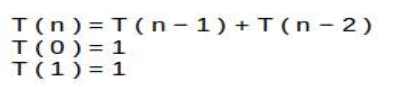
\includegraphics[scale=1]{images/4c.png}
    % \caption{Caption}
    \label{fig:my_label}
\end{figure}
Xét phương trình T(n) - T(n-1) - T(n-2) = 0 \\
\text{Đặt} X^n = T(n) \\
\text{Ta có:} X^n - X^{n-1} - X^{n-2} = 0 \\
\text{Phương trình đặc trưng:} X^2 - X - 1 = 0 \\
=> 
\begin{cases}
    X_1 = \frac{1+\sqrt{5}}{2} \\
    X_2 = \frac{1-\sqrt{5}}{2}
\end{cases}
\\
\text{Ta có: T(n) = } $c_1X_1^n + c_2X_2^n$ = $c_1(\frac{1+\sqrt{5}}{2})^n + c_2(\frac{1-\sqrt{5}}{2})^n$ \\
\begin{cases}
    T(0) = 1\\
    T(1) = 1
\end{cases}
=>
\begin{cases}
    c_1 + c_2 = 1\\
    \frac{1}{2}(c_1+c_2) + \frac{\sqrt{5}}{2}(c_1-c_2) = 1
\end{cases}
=>
\begin{cases}
    c_1 + c_2 = 1\\
    c_1-c_2 = \frac{1}{\sqrt{5}}
\end{cases}
=>
\begin{cases}
    c_1 = \frac{1}{2} + \frac{1}{2\sqrt{5}}\\
    c_2 = \frac{1}{2} - \frac{1}{2\sqrt{5}}
\end{cases}
\textbf{Vậy:} 
T(n) = ${({\frac{1}{2} + {\frac{1}{2\sqrt{5}}})({\frac{1+\sqrt{5}}{2})}^n}} + {(\frac{1}{2} - \frac{1}{2\sqrt{5}})({\frac{1-\sqrt{5}}{2})}^n}$
% Bai 5
\section*{Bài tập 5: Giải phương trình đệ quy sau dùng phương pháp hàm sinh} 
\addcontentsline{toc}{section}{Bài tập 5: Giải phương trình đệ quy sau dùng phương pháp hàm sinh}
\subsection*{a)}
\addcontentsline{toc}{subsection}{a)}
\begin{figure}[H]
    \centering
    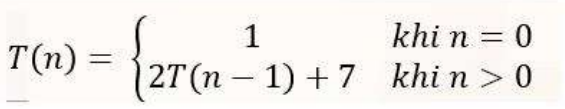
\includegraphics[scale=1.2]{images/5a.png}
    % \caption{Caption}
    \label{fig:my_label}
\end{figure}
Hàm sinh của dãy vô hạn {T(n)}$_{n=0\to\infty}$ có dạng: \\
f(x) $= \sum_{n=0}^{\infty}{T(n)x^n} = \sum_{n=1}^{\infty}{[2T(n-1)+7]x^n+1} = 2\sum_{n=1}^{\infty}{T(n-1)x^n} + 7\sum_{n=1}^{\infty}{x^n} + 1$ \\
Đặt A = $\sum_{n=1}^{\infty}{T(n-1)x^n}$, B = $7\sum_{n=1}^{\infty}{x^n}$\\
A = $\sum_{n=1}^{\infty}{T(n-1)x^n} = x\sum_{n=1}^{\infty}{T(n-1)x^{n-1}} = xf(x)$\\
B = $7\sum_{n=1}^{\infty}{x^n} = 7\big(\frac{1}{1-x}-1\big)$\\
\textbf{Khi đó: }
f(x) = $2xf(x) + 7\big(\frac{1}{1-x}-1\big) + 1 = 2xf(x) + \frac{7}{1-x} -6 \\
\Rightarrow f(x) = \frac{6x+1}{(1-x)(1-2x)} = \frac{a}{1-x}+ \frac{b}{1-2x} \\
\Rightarrow a(1-2x) + b(1-x) = 6x+1
\Rightarrow
\begin{cases}
    a + b =1 \\
    -2a-b = 6 
\end{cases}
\Rightarrow
\begin{cases}
    a = -7 \\
    b = 8
\end{cases}\\
\Rightarrow f(x) = \frac{-7}{1-x} + \frac{8}{1-2x} = -7\sum_{n=0}^{\infty}{x^n} + 8\sum_{n=0}^{\infty}{(2x)^n} = \sum_{n=0}^{\infty}{(-7+8.2^n)x^n}\\$
Vậy T(n) = -7 + 8.$2^n$
\subsection*{b)}
\addcontentsline{toc}{subsection}{b)}
\begin{figure}[H]
    \centering
    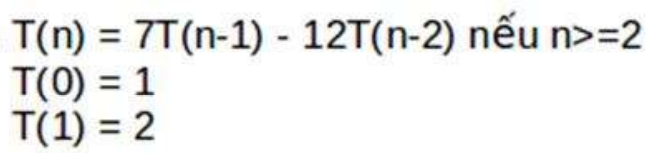
\includegraphics[scale=1]{images/5b.png}
    % \caption{Caption}
    \label{fig:my_label}
\end{figure}
Hàm sinh của dãy vô hạn {T(n)}$_{n=0\to\infty}$ có dạng: \\
f(x) $= \sum_{n=0}^{\infty}{T(n)x^n} = \sum_{n=1}^{\infty}{[7T(n-1)-12T(n-2)]x^n+1+2x} = 7\sum_{n=1}^{\infty}{T(n-1)x^n} - 12\sum_{n=1}^{\infty}{T(n-2)x^n} + 1 + 2x$ \\
Đặt A = $\sum_{n=2}^{\infty}{T(n-1)x^n}$, B = $\sum_{n=2}^{\infty}{T(n-2)x^n}$\\
A = $\sum_{n=2}^{\infty}{T(n-1)x^n} = x\sum_{n=2}^{\infty}{T(n-1)x^{n-1}} = xf(x)$\\
B = $x^2\sum_{n=2}^{\infty}{T(n-2)x^n} = x^2f(x)$\\
\textbf{Khi đó: }
f(x) = $7x(f(x)-1) + 12x^2f(x) + 1 +2x = 7xf(x) -7x -12x^2f(x) +1+2x \\
\Rightarrow f(x) = \frac{1-5x}{1-7x+12x^2} = \frac{-8}{x-1/3}+ \frac{3}{x-1/4}= \frac{24}{1-3x}- \frac{12}{1-4x} \\
\Rightarrow f(x) = \sum_{n=1}^{\infty}{24(n-1)3^nx^n} + \sum_{n=0}^{\infty}{(12(n-1)4^nx^n} = \sum_{n=0}^{\infty}{12(n-1)(12.{3}^n-4^n)x^n}\\$
Vậy T(n) = $12(n-1)(12.{3}^n-4^n)$
\subsection*{c)}
\addcontentsline{toc}{subsection}{c)}
\begin{figure}[H]
    \centering
    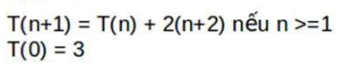
\includegraphics[scale=1]{images/5c.png}
    % \caption{Caption}
    \label{fig:my_label}
\end{figure}
Đặt n = t - 1, ta có: \\
\begin{cases}
    T(t) = T(t-1) + 2(t+1), \text{nếu t \geq 2} \\
    T(0) = 3 \\
    T(1) = 7
\end{cases}
Hàm sinh của dãy vô hạn ${T(n)}_{0\to\infty}$ là: \\ 
\text{f(x)} = $\sum_{t=0}^{\infty}{T(t)x^t}$ = $\sum_{t=2}^{\infty}{T(t)x^t} + T(1).x^1 + T(0).x^0$ 
= $\sum_{t=2}^{\infty}{T(t-1)+2(t+1)} + 7x + 3$ \\
&= $\sum_{t=2}^{\infty}{T(t-1)x^t} + 2\sum_{t=2}^{\infty}{(t+1)x^t} + 7x + 3$ \\
&= $xf(x) - 3x + 2[\frac{1}{(1-x)^2} - 1 - 2x] + 7x + 3$ = $xf(x) + 1 + \frac{2}{(1-x)^2}$
=> $(1-x)f(x)=1 + \frac{2}{(1-x)^2}$ => $f(x)=\frac{1}{(1-x)}+\frac{2}{(1-x)^3}$ 
 = $\sum_{t=0}^{\infty}{x^t} + 2\sum_{t=0}^{\infty}{\frac{(t+2)!}{t!.2!}x^t}$ 
 &= $\sum_{t=0}^{\infty}{[1 + (t+1)(t+2)]x^t}$ \\
 \text{mà f(x) = $\sum_{t=0}^{\infty}{T(t)x^t}$} => $T(t)=t^2+3t+4$
% Bài 6
\section*{Bài tập 6: Phương pháp đoán nghiệm} 
\addcontentsline{toc}{section}{Bài tập 6: Phương pháp đoán nghiệm}
\begin{figure}[H]
    \centering
    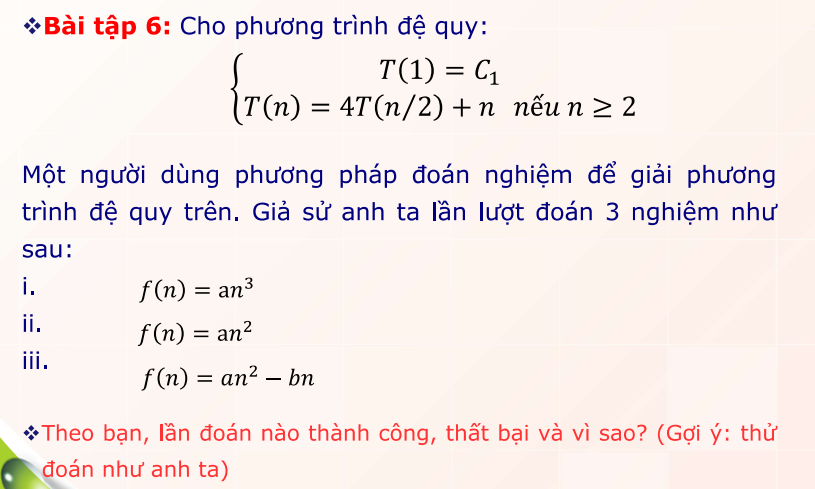
\includegraphics[scale=.7]{images/6.png}
    % \caption{Caption}
    \label{fig:my_label}
\end{figure}

% i
\textbf{i.} \\
\underline{B1}: CM: T(1) $\leq$ f(1) \\
Với n =1, T(1) = C1 và f(1) = a \\
Để có T(1) $\leq$ f(1) thì chọn C1 $\leq$ a (1)\\
\underline{B2}: Giả sử T(k) $\leq$ f(k), $\forall$ k< n \\
\underline{B3}: Ta CM T(n) $\leq$ f(n), $\forall$ n \\
Áp dụng giả thiết quy nạp với k = $\frac{n}{2}$ < n (n > 0)\\
Ta có T(n/2) $\leq$ f(n/2) = $\frac{an^3}{8}$ \\
T(n) = 4T(n/2) + n $\leq \frac{an^3}{2}$ + n \\
$\Rightarrow$ T(n) $\leq \frac{an^3}{2}$ + n = f(n) - $\frac{an^3}{2}$ + n \\
Nếu $\frac{-an^3}{2}$ + n $\leq$ 0 $\Rightarrow$ T(n) $\leq$ f(n) -$\frac{an^3}{2}$ + n $\leq$ f(n) \\
Có $\frac{-an^3}{2}$ + n $\leq$ 0 $\Leftrightarrow \frac{-1}{2}n(an^2 -2) \leq 0 \Rightarrow an^2 -2 \geq 0$ (vì n>0) $\Leftrightarrow$ a $\geq \frac{2}{n^2}$  \\
$\frac{2}{n^2}$ đạt GTLN tại n = 1 $\Rightarrow \frac{2}{n^2} \leq$ 2 ($\forall$ n > 0) (2) \\
(1), (2) $\Rightarrow$ nếu chọn a = |C1| + 2 thì: 
$\begin{cases}
    |C1| + 2 = a \geq \frac{2}{n^2} \\
    C1 \leq a = |C1| + 2
\end{cases} \\
\Rightarrow$ T(n) $\leq (|C1| + 2) n^3 $ $\forall n \\
\Rightarrow$ T(n) = O($n^3$) \\
% ii
\textbf{ii.} \\
\underline{B1}: CM: T(1) $\leq$ f(1) \\
Với n =1, T(1) = C1 và f(1) = a \\
Để có T(1) $\leq$ f(1) thì chọn C1 $\leq$ a (1)\\
\underline{B2}: Giả sử T(k) $\leq$ f(k), $\forall$ k< n \\
\underline{B3}: Ta CM T(n) $\leq$ f(n), $\forall$ n \\
Áp dụng giả thiết quy nạp với k = $\frac{n}{2}$ < n (n > 0)\\
Ta có T(n/2) $\leq$ f(n/2) = $\frac{an^2}{4}$ \\
T(n) = 4T(n/2) + n $\leq an^2$ + n \\
$\Rightarrow$ T(n) $\leq an^2$ + n = f(n) + n \\
Nếu  n $\leq$ 0 $\Rightarrow$ T(n) $\leq$ f(n) + n $\leq$ f(n) \\
mà  n $\leq$ 0 $\Rightarrow$ vô lý  \\
$\frac{2}{n^2}$ đạt GTLN tại n = 1 $\Rightarrow \frac{2}{n^2} \leq$ 2 ($\forall$ n > 0) (2) \\
=> đoán nghiệm f(x) = $an^2$ là không đúng.\\
% iii
\textbf{iii.} \\
\text{Với $n = 1$ , $T(1) = c_1$ , $f(1) = a - b$} \\
\text{Để có $T(1) \leq f(1)$ => chọn $ c_1 \leq a - b$ } \\
\text{Giả sử $T(k) \leq f(k)$ $\forall k< n$}  \\
\text{Ta chứng minh: } $T(n)\leq f(n)$ $\forall {n}$  \\
\text{Áp dụng giả thiết quy nạp với $k = \frac{n}{2} < n (n>1)$} \\
\text{Ta có: }\\
$T(\frac{n}{2}) \leq f(\frac{n}{2})$ = $a\frac{n^2}{4} - b\frac{n}{2}$ \\
=> $4T(\frac{n}{2}) + n \leq an^2-2bn+n$ \\
=> $T(n) \leq an^2-2bn+n = f(n)-bn+n$ \\
\text{Nếu $n-bn \leq 0 => T(n) \leq f(n)$} \\
\text{Ta thấy $n-bn \leq 0 <=> n(1-b) \leq 0 \text{ vì } n > 0 => b\geq1$}
\text{Ta có hệ:}
\begin{cases}
    b \geq 1 \\
    a-b \geq c_1
\end{cases} \\
Chọn b=1; a = c_1 + 1 => $T(n) \leq (c_1 + 1)n^2 - n$ $\forall n$ \\
=> $T(n) = O(n^2)$
% Bài 7
\section*{Bài tập 7: Phương pháp đoán nghiệm} 
\addcontentsline{toc}{section}{Bài tập 7: Phương pháp đoán nghiệm}
\begin{figure}[H]
    \centering
    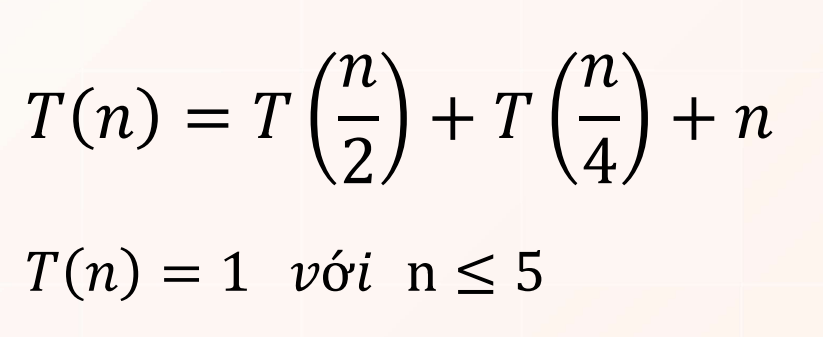
\includegraphics[scale=.7]{images/7.png}
    % \caption{Caption}
    \label{fig:my_label}
\end{figure}
Đoán f(n) = an + b \\
Dùng quy nạp để CM: T(n) $\leq$ f(n), $\forall$ n \\
\underline{B1}: CM: T(n) $\leq$ f(n) với n $\leq$ 5 \\
Với n =0, T(0) = 1 và f(0) = b \\
Với n =1, T(1) = 1 và f(1) = a+b \\
Với n =2, T(2) = 1 và f(2) = 2a+b\\
...\\
Để có T(n) $\leq$ f(n) với n $\leq$ 5 thì chọn b = 1, a $\geq$ 0\\
\underline{B2}: Giả sử T(k) $\leq$ f(k), $\forall$ k< n \\
\underline{B3}: Ta CM T(n) $\leq$ f(n), $\forall$ n > 5\\
Áp dụng giả thiết quy nạp với $k_1$ = $\frac{n}{2}$ < n\\
Ta có T(n/2) $\leq$ f(n/2) = $\frac{an}{2}$ + b (1)\\
Áp dụng giả thiết quy nạp với $k_2$ = $\frac{n}{4}$ < n \\
Ta có T(n/4) $\leq$ f(n/4) = $\frac{an}{4}$ + b (2)\\
(1), (2) $\Rightarrow$ T(n/2) + T(n/4) + n $\leq \frac{an}{2}$ + b + $\frac{an}{4}$ + b + n \\
$\Rightarrow$ T(n) $\leq \frac{3an}{4}$ + 2b + n = f(n) - $\frac{an}{4}$ + b + n\\
Nếu - $\frac{an}{4}$ + b + n $\leq$ 0 $\Rightarrow$ T(n) $\leq$ f(n) - $\frac{an}{4}$ + b + n $\leq$ f(n) \\
 - $\frac{an}{4}$ + b + n $\leq$ 0 $\Rightarrow$ - $\frac{an}{4}$ + 1 + n $\leq$ 0 $\Rightarrow a \geq 4 + \frac{4}{n}$ \\
 Có 4 + $\frac{4}{n}$ đạt GTLN tại n = 6 (với n > 5)$\Rightarrow 4 + \frac{4}{n} \leq \frac{14}{3}$ ($\forall$ n > 5)\\
 Vậy nếu chọn a = 14/3 thì 14/3 = a $\geq 4 + \frac{4}{n}$ \\
 a = 14/3, b = 1 $\Rightarrow$ T(n) $\leq \frac{14}{3}$ n + 1 $\forall$ n \\
  $\Rightarrow$ T(n) = O(n)
\end{document}